\documentclass[14pt, openany]{article}
\usepackage[utf8]{inputenc}
\usepackage[T1]{fontenc}
\usepackage{hyperref}
\usepackage[french]{babel}
\frenchbsetup{StandardLists=true}
\usepackage{amsmath,amsfonts,amssymb}
\usepackage{graphicx}
\usepackage[a4paper,left=2cm,right=2cm,top=2cm,bottom=2cm]{geometry}
\usepackage{bbm}
\usepackage{libertine}
\usepackage{color}
\usepackage{array,multirow,makecell}
\usepackage{enumitem} %Pour modifier les puces
\usepackage{caption}
\usepackage{dsfont}
\usepackage{algorithm}
\usepackage{algorithmic}
%%% francisation des algorithmes :
\renewcommand{\algorithmicrequire}{\textbf{Entrées : }}
\renewcommand{\algorithmicensure}{\textbf{Début}}
\renewcommand{\algorithmicreturn}{\textbf{Retourner}}
\renewcommand{\algorithmicwhile}{\textbf{tant que}}
\renewcommand{\algorithmicdo}{\textbf{}}
\renewcommand{\algorithmicprint}{\textbf{Fin}}
\renewcommand{\algorithmicfor}{\textbf{Pour}}
\renewcommand{\algorithmicendfor}{\textbf{Fin pour}}
\renewcommand{\algorithmicendwhile}{\textbf{Fin du \og Tant que\fg }}

\newcolumntype{R}[1]{>{\raggedleft\arraybackslash }b{#1}}
\newcolumntype{L}[1]{>{\raggedright\arraybackslash }b{#1}}
\newcolumntype{C}[1]{>{\centering\arraybackslash }b{#1}}
\setlength{\parindent}{0cm}
\setlength{\parskip}{1ex plus 0.5ex minus 0.2ex}
\newcommand{\hsp}{\hspace{20pt}}
\newcommand{\HRule}{\rule{\linewidth}{0.5mm}}
\AddThinSpaceBeforeFootnotes
\FrenchFootnotes

%%%% debut macro %%%%
\newenvironment{changemargin}[2]{\begin{list}{}{%
\setlength{\topsep}{0pt}%
\setlength{\leftmargin}{0pt}%
\setlength{\rightmargin}{0pt}%
\setlength{\listparindent}{\parindent}%
\setlength{\itemindent}{\parindent}%
\setlength{\parsep}{0pt plus 1pt}%
\addtolength{\leftmargin}{#1}%
\addtolength{\rightmargin}{#2}%
}\item }{\end{list}}
%%%% fin macro %%%%

\begin{document}

\begin{titlepage}
\begin{center}
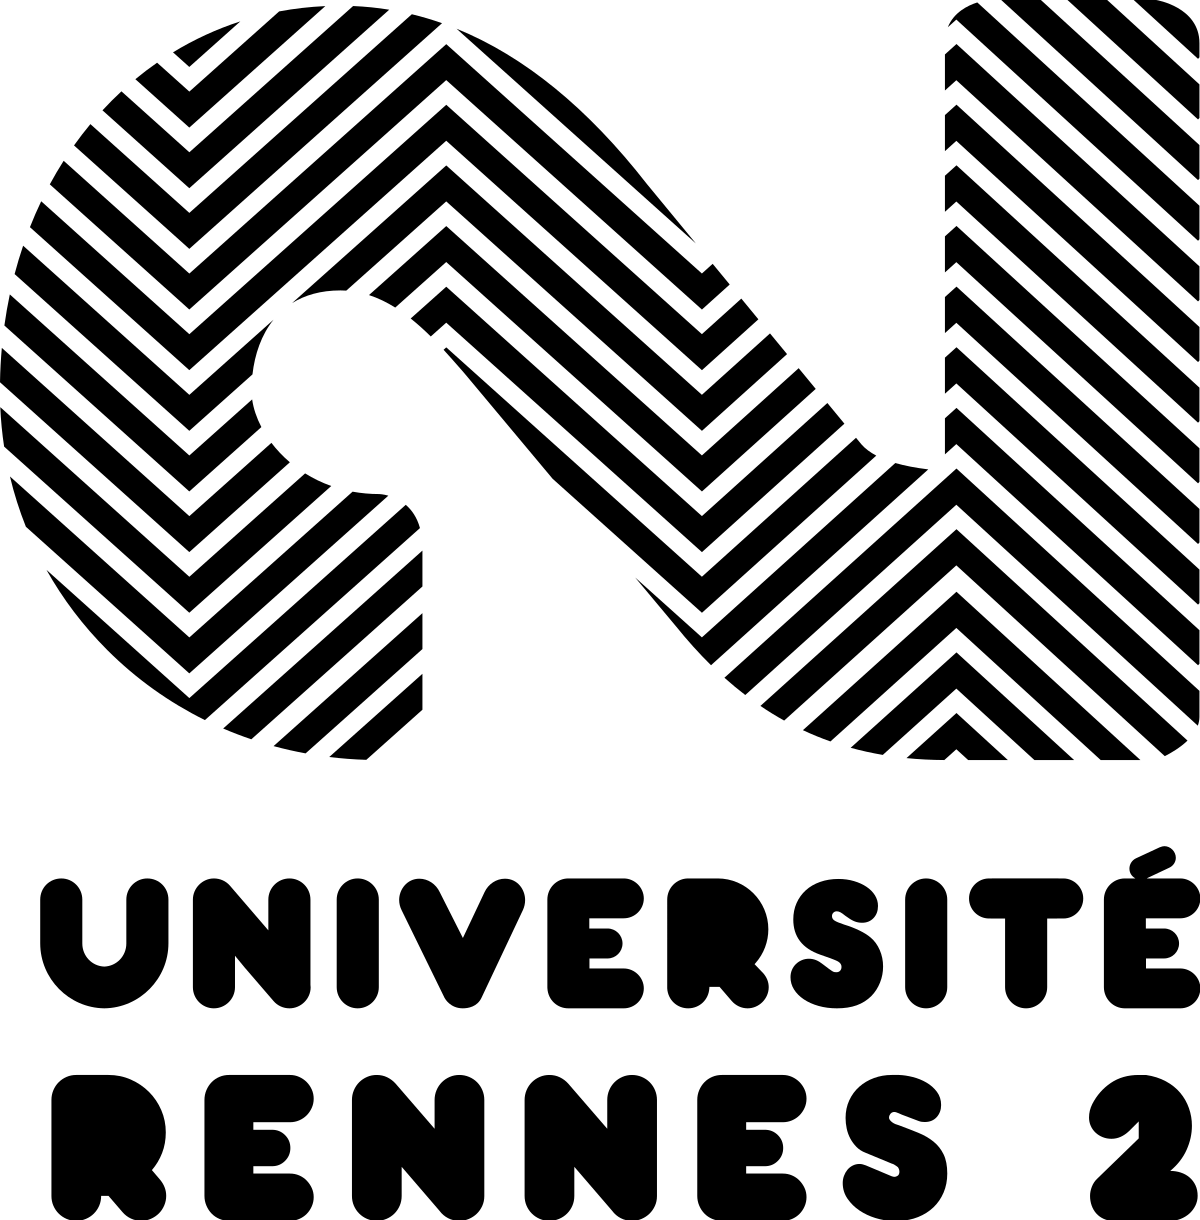
\includegraphics[scale=0.15]{Images/ur2.png}\\
\bigskip
\textsc{\Large PROJET DATA SCIENCE - MASTER 2 MAS PARCOURS SCIENCES DES DONNEES\\ 
\bigskip
Rapport de l'étude}\\
\bigskip
    \HRule \\[0.4cm]
    { \huge \bfseries Prédictions des températures de 7 stations différentes à un horizon de 36 heures\\[0.4cm] }
        \HRule \\[2cm]
   \begin{figure}[h]
    \begin{minipage}[c]{.46\linewidth}
        \centering
        
\includegraphics[scale=0.3]{Images/defi.png}
    \end{minipage}
    \hfill%
    \begin{minipage}[c]{.46\linewidth}
        \centering
        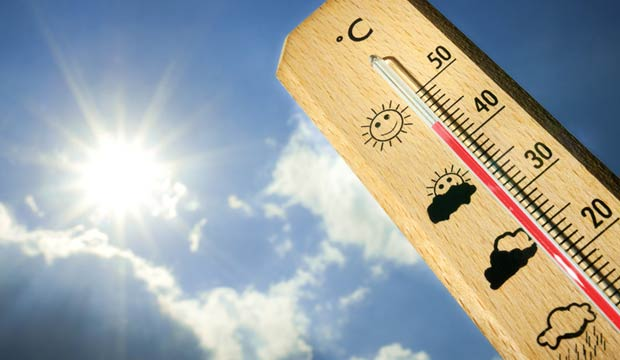
\includegraphics[scale=0.36]{Images/temp.jpg}
    \end{minipage}
	\end{figure}
    \bigskip
    \begin{minipage}{0.4\textwidth}
      \begin{flushleft} \large
      \emph{Team :} \textsc{Freak-unit}\\
      \emph{Membres :}
      \begin{itemize}
      	\item \textsc{Benjamin ALLEAU}\\
      	\item \textsc{Abdessamad AZNAGUE}\\
        \item \textsc{Guillaume LE FLOCH}\\
      \end{itemize}
      \end{flushleft}
    \end{minipage}
    \begin{minipage}{0.4\textwidth}
      \begin{flushright} \large
      	\emph{Organisateur :} \textsc{INSA de Toulouse}
        \emph{Encadrant :} \textsc{M. Romain TAVENARD}\\         
      \end{flushright}
    \end{minipage}

    \vfill
    
    % Bottom of the page
    {\large 05 Octobre 2017 —  08 Janvier 2018}

\end{center}
\end{titlepage}

\renewcommand{\contentsname}{Plan}

\tableofcontents
\newpage

\section{Présentation du projet}
\paragraph{}
La compétition 2017-2018 est basée sur une stratégie d'adaptation statistique pour améliorer la prévision de températures à un horizon de 36 heures.

Les services du \textbf{CNRM} (Centre National de Recherches Météorologiques) construisent des grands modèles déterministes de l'atmosphère par résolution des équations de Navier et Stockes sur un maillage: 10km pour \textbf{ARPEGE}, kilométrique pour \textbf{AROME} mais limité à l'Europe. Il apparaît que ces modèles sont généralement biaisés, notamment parce qu'ils ne peuvent prendre en compte des phénomènes à petite échelle. Par exemple, un vent important (e.g. vent d'autan à Toulouse) provoque des turbulences qui, en mélangeant les couches d'air, entrainent une baisse de la température par rapport à celle prévue.

Un modèle statistique intégrant les prévisions du modèle déterministe peut contribuer à réduire significativement ces biais. En revanche, un modèle statistique seul est incapable de prévoir l'arrivée d'une perturbation océanique à partir de données locales. L'adaptation statistique est donc une mise en collaboration \og optimale \fg{} des deux approches de modélisation, déterministe et statistique.

Le \og Défi Grosses Data \fg{} est donc un challenge mettant en confrontation une multitude de groupes d'étudiants provenant des \textbf{INSA} de Toulouse et Rennes, ainsi que des Universités de \textbf{Bordeaux}, \textbf{Rennes 1}, \textbf{Rennes 2}, \textbf{Paris Descartes}, \textbf{Paul Sabatier (Toulouse 3)} ou encore la \textbf{Toulouse School of Economics}. Ce rapport détaillera le travail fourni par l'équipe \textbf{Freak-unit}, une des 8 équipes représentant l'\textbf{Université de Rennes 2}.

L'objectif de ce projet est simple : prédire au mieux les températures de 7 stations sur un horizon de 36 heures. Pour ce faire, 36 fichiers $train\_H.csv$ $(H=1,..,36)$, ont été mis à notre disposition. Ces fichiers contiennent les variables issues des modèles physiques décrits dans le préambule à un horizon de +H heures. Leur contenu est le suivant :
\begin{itemize}
\item les lignes correspondent à chaque jour sur une période allant du $1^{er}$ janvier 2014 au 30 mai 2016.
\item les colonnes contiennent 30 variables (température, nébulosité, vent, humidité ..)
\end{itemize}
Nous allons détailler ces variables afin de bien comprendre quelles sont les mesures à notre disposition :
\begin{itemize}
\item \textbf{insee} : Facteur à 7 niveaux représentant le numéro insee des stations pour lesquelles nous cherchons à prédire les températures (Nice, Toulouse Blagnac, Bordeaux-Mérignac, Rennes, Lille Lesquin, Strasbourg Entzheim, Paris-Montsouris)
\item \textbf{tH2\_obs} : Observation de la température à 2 mètres \textit{in situ} au point station (prédictant). \textbf{C'est la variable réponse que l'on cherche à prédire}
\item \textbf{ech} : Facteur à 36 niveaux correspondant à l'échéance de validité (H)
\item \textbf{capeinsSOL0} : Energie potentielle convective
\item \textbf{ciwcH20} : Fraction de glace nuageuse à 20 mètres
\item \textbf{clwcH20} : Fraction d'eau nuageuse à 20 mètres
\item \textbf{nH20} : Fraction nuageuse à 20 mètres
\item \textbf{pMER0} : Pression au niveau de la mer
\item \textbf{rr1SOL0} : Précipitation horaire au niveau du sol
\item \textbf{rrH20} : Précipitation horaire à 20 mètres
\item \textbf{tpwHPA850} : Température potentielle au niveau 850 hPa
\item \textbf{ux1H10} : Rafale 1 minute du vent à 10 mètres composante zonale
\item \textbf{vapcSOL0} : Colonne de vapeur d'eau
\item \textbf{vx1H10} : Rafale 1 minute du vent à 10 mètres composante verticale
\item \textbf{ddH10\_rose4} : Facteur à 4 niveaux indiquant la direction du vent à 10 mètres (en rose4)
\item \textbf{ffH10} : Force du vent à 10 mètres en m/s
\item \textbf{flir1SOL0} : Flux Infra-rouge en J/$m^2$
\item \textbf{fllat1SOL0} : Flux de chaleur latente en J/$m^2$
\item \textbf{flsen1SOL0} : Flux de chaleur sensible en J/$m^2$
\item \textbf{flvis1SOL0} : Flux visible en J/$m^2$
\item \textbf{hcoulimSOL0} : Hauteur de la couche limite en mètres
\item \textbf{huH2} : Humidité 2mètres en \%
\item \textbf{iwcSOL0} : Réservoir neige kg/$m^2$ (équivalent en eau liquide des chutes de neige
\item \textbf{nbSOL0\_HMoy} : Nébulosité basse (moyenne sur les 6 points de grille autour de la station) (fraction en octat du ciel occulté)
\item \textbf{ntSOL0\_HMoy} : Nébulosité totale (moyenne sur les 6 points de grille autour de la station)
\item \textbf{tH2} : Température à 2 mètres du modèle \textbf{AROME}
\item \textbf{tH2\_VGrad\_2.100} : Gradient vertical de température entre 2 mètres et 100 mètres
\item \textbf{tH2\_XGrad} : Gradient zonal de température à 2 mètres
\item \textbf{tH2\_YGrad} : Gradient méridien de température à 2 mètres
\item \textbf{mois} : Facteur à 12 niveaux représentant le mois
\end{itemize}
Il est à noter que ces 36 fichiers \textit{train} contiennent des valeurs manquantes, le sujet sera approfondi un peu plus tard dans l'étude.

L'objectif de ce projet est le suivant : à partir des différents fichiers \textit{train} nous devons réaliser un apprentissage (supervisé dans notre cas) afin de pouvoir appliquer par la suite notre modèle au fichier \textit{test.csv} qui contient les mêmes variables, à l'exception de \textbf{tH2\_obs} évidemment puisqu'il faut la prédire. Les lignes du fichier \textit{test.csv} contiennent les 6 périodes de 15 jours suivantes :
\begin{itemize}
\item du 20/06/2016 au 02/07/2016
\item du 01/08/2016 au 14/08/2016
\item du 12/09/2016 au 25/09/2016
\item du 24/10/2016 au 06/11/2016
\item du 05/12/2016 au 18/12/2016
\item du 08/05/2017 au 21/05/2017
\end{itemize}
Une fois les prédictions effectuées, il faut soumettre les résultats sous forme d'un fichier au format \textit{csv} toujours, sur le site internet du challenge. Au bout d'exactement 1 heure après la soumission, nous pouvons visualiser notre score. La métrique utilisée pour évaluer le score est le \textbf{RMSE} (Root Mean Square Error). Si l'on note $\hat{y}$ notre vecteur de prédictions et $y_{obs}$ les valeurs des températures réellement observées, le \textbf{RMSE} associé se note :\\
\begin{center}
$RMSE_{\hat{y}} = \sqrt{\frac{1}{n} \sum\limits_{i=1}^n (\hat{y_i}-y_{obs_i})^2}$
\end{center}
En d'autres termes, cette métrique permet de mesurer d'une certaine façon l'écart entre nos prédictions et la réalité. Il est à noter que le challenge fournit un score de $1.30755$ appelé \textbf{Baseline} qui correspond à un score de référence, associé à \og un modèle élémentaire de prévision sans effort particulier d'optimisation. C'est un objectif a minima à améliorer dans ce concours \fg{}. Le décor est planté, désormais il ne reste plus qu'à se lancer dans le challenge.
\section{Remerciements}
\paragraph{}
Avant de détailler les différentes étapes de ce projet, les 3 membres de la \textbf{Freak-unit} team souhaitent remercier tout particulièrement leur professeur encadrant, \textbf{M. Romain TAVENARD} pour son accompagnement tout au long du projet et pour l'aide apportée. Sa connaissance du \textit{Deep Learning} aura notamment été un facteur déterminant dans la réalisation de ce projet.

\section{Différentes stratégies envisagées}
\paragraph{}
Afin d'effectuer l'analyse la plus fine et pertinente possible, il est primordial de bien définir la stratégie d'étude à adopter. Par \og stratégie \fg{}, nous parlons ici de la façon dont nous allons structurer les données et des techniques que nous allons employer pour optimiser la performance des algorithmes. Cela peut être vu comme un problème d'optimisation sous contrainte : notre objectif est de réaliser la meilleure performance sous des contraintes de temps et de matériel. Il faut donc réussir à combiner au mieux la théorie mathématique avec la réalisation informatique.

\subsection{Structuration des données}
\paragraph{}
Un premier travail a consisté à agréger les données des 36 fichiers $train\_H.csv$ $(H=1,..,36)$ dans un seul jeu de données : cela aboutit à une matrice de $189 281$ lignes et $31$ colonnes. Dans un deuxième temps, nous avons divisé ce fichier en $7$ sous-fichiers : un fichier regroupant les prédictions aux 36 échéances de chaque station. Ce choix a été guidé par 3 éléments :
\begin{itemize}
\item L'intuition : sachant qu'il existe plusieurs types de climats (océaniques, continental, méditerranéen) et qu'on les retrouve à travers les stations présentes dans les données, il ne paraît pas anormal d'essayer de prédire chaque station indépendamment des autres. Ne perdons pas de vue que les chiffres sont là pour quantifier la réalité, l'objectif est donc de les utiliser pour représenter au mieux les phénomènes réels.
\item Un indice lâché par les organisateurs du concours qui ont laissé entendre qu'il pouvait exister un biais lié à chaque station.
\item L'analyse du comportement des indicateurs par station.
\end{itemize}
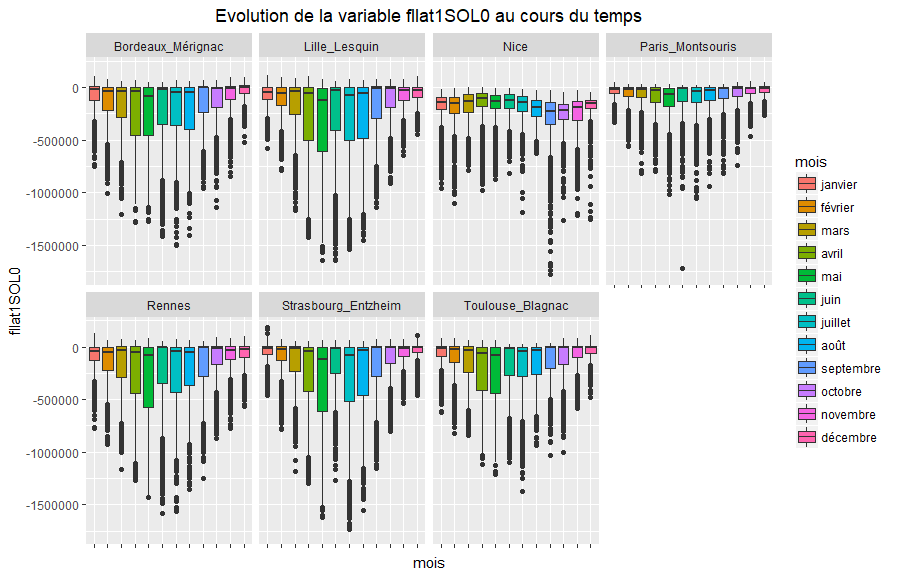
\includegraphics[width=17cm]{Images/fllat.png}
\begin{center}
\captionof{figure}{Exemple du flux de chaleur latente dont le comportement diffère d'une station à une autre}
\label{fig1}
\end{center}
\paragraph{}
Dans la suite, nous verrons que le gros jeu de données ($189281$ lignes) ou les fichiers par stations seront utilisés en fonction de l'algorithme choisi. Une autre option aurait pu être de découper les données par station et par échéance. Cependant en procédant de la sorte, on se retrouverait avec 252 modèles à estimer, et l'on s'exposerait également au risque de sur-apprentissage (\textit{overfitting} en anglais). La dimension des données va également impacter le choix de la méthode d'estimation des paramètres et d'estimation de la performance de l'algorithme : la \textbf{validation croisée}. Nous allons donc effectuer quelques rappels sur ces différents concepts.

\subsection{Notions d'overfitting/underfitting}
\paragraph{}
Comme introduit brièvement un peu plus haut dans ce rapport, l'un des enjeux de ce projet dans le but d'obtenir les meilleures prédictions possibles, selon le critère du \textbf{RMSE}, et donc d'éviter de se retrouver en situation sur-apprentissage ou de sous-apprentissage (respectivement \textit{overfitting} et \textit{underfitting}). En ce sens, on va chercher à construire un estimateur (une fonction) optimal, robuste qui conservera un pouvoir de prédiction de qualité sur un nouvel échantillon. Prenons le dessin suivant qui sera un peu plus parlant.
\paragraph{}
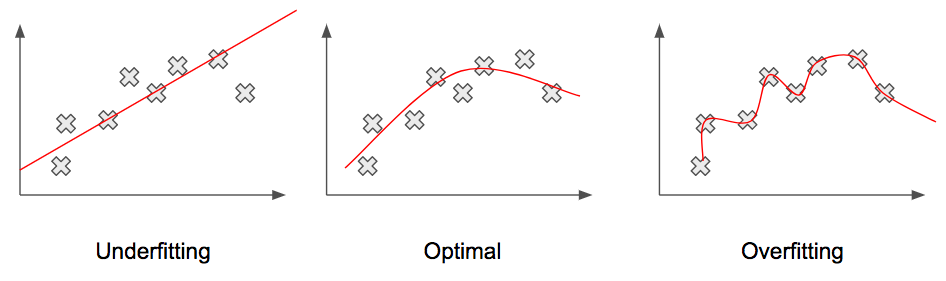
\includegraphics[width=17cm]{Images/overfitting.png}
\begin{center}
\captionof{figure}{Illustration de ces notions à partir d'un exemple simple dans $\mathbb{R}^2$}
\label{fig1}
\end{center}
On s'aperçoit que sur le graphe de gauche, l'estimateur est trop rigide, il ne \og colle \fg{} pas assez aux données. Sur le graphe de droite c'est le contraire, l'estimateur est beaucoup trop sensible aux valeurs, et lorsque les données changeront, les prédictions ne seront donc plus aussi précises. Nous souhaitons donc trouver une fonction ayant une allure similaire à celle du graphe du milieu, qui sera plus \og robuste \fg{} que les deux autres.


Nous verrons dans la suite que pour remédier au problème de l'overfitting, nous pouvons utiliser des formes de \textbf{régularisation}, encore appelées pénalités et qui se traduiront par des contraintes dans le problème d'optimisation d'une certaine \textbf{fonction de perte} que l'on va choisir.\\

Une façon de vérifier que le modèle est robuste peut-être de procéder à de la \textbf{validation croisée}, c'est donc le prochain point que nous allons développer.
 
\subsection{Validation croisée}
\paragraph{}
Comme énoncé précédemment, nous allons utiliser des méthodes de validation croisée à la fois pour contrôler la performance et la robustesse de l'algorithme mis en œuvre, mais également pour calibrer des hyper-paramètres dans le cas de modèles complexes. Nous allons donc dans la suite effectuer quelques rappels théoriques afin de bien comprendre pourquoi nous utilisons ces méthodes ainsi qu'une présentation des deux types de validation croisée que nous avons choisi d'employer.

\subsubsection{Contexte théorique}
\paragraph{}
Soit $d^{n}_{1}$ l'observation d'un n-échantillon $D^{n}_{1} =$\{$(X_1,Y_1),...,(X_n,Y_n)$\} d'une loi conjointe $P$ sur $\mathcal{X}$ x $\mathcal{Y}$ qui est inconnue. On cherche à estimer cette loi $P$ à l'aide des données disponibles, à savoir $d^{n}_{1}$. En théorie, il faudrait minimiser la quantité appelée \textbf{risque} (ou encore \textbf{erreur de généralisation}) d'une règle de prédiction que l'on va noter $f$. Ainsi de façon mathématique, on définit le \textbf{risque} de la manière suivante :
\paragraph{}
$\mathcal{R}_P(f) = \mathbb{E}_{(X,Y)}[l(Y,f(X))]$ avec $l$ que l'on appelle \textbf{fonction de perte} et qui a pour expression :
\begin{itemize}
\item $l(y,y') = |y-y'|^q$ en régression réelle (on prendra souvent la perte \textit{quadratique}, c'est-à-dire lorsque $q=2$)
\item $l(y,y') = \mathds{1}_{y \neq y'}$ en discrimination binaire.
\end{itemize}
\paragraph{}
Cependant en pratique, il nous est impossible de calculer le \textbf{risque}, $P$ étant inconnue. Il faut donc l'estimer et chercher à minimiser cette quantité estimée par la suite. Une première approche naturelle serait d'utiliser le risque empirique, c'est-à-dire d'estimer l'espérance de la fonction de perte par la moyenne empirique de cette même fonction. Le \textbf{risque empirique} d'un algorithme de prédiction $f_{D^{n}_{1}}$ construit sur $D^{n}_{1}$ se note de la façon suivante :
\begin{center}
$\widehat{\mathcal{R}}_n(f_{D^{n}_{1}}) = \frac{1}{n} \sum\limits_{i=1}^n l(Y_i,f_{D^{n}_{1}}(X_i))$
\end{center}

\paragraph{}
Le problème de cet estimateur est l'absence d'indépendance : en effet, pour effectuer ses prédictions il se sert des mêmes données qui ont servi à faire l'algorithme d'apprentissage. En ce sens, notre algorithme risque de trop \og coller \fg{} aux données d'apprentissage, puisqu'il aura acquis l'information à partir de ces données il sera capable de bien prédire la variable réponse, mais risque de ne pas être aussi performant à l'avenir sur un nouveau jeu de données. C'est ce qu'on nous avons défini comme étant l'\textit{overfitting}. C'est donc pour corriger ce problème que nous allons avoir recours à d'autres méthodes d'estimation du \textbf{risque}, qui sont meilleures : les méthodes de \textbf{validation croisée}.

\subsubsection{La validation croisée Hold-Out}
\paragraph{}
Le concept de base pour la validation croisée \textbf{Hold-Out} consiste à séparer nos données $d^{n}_{1}$ en deux sous-échantillons :
\begin{itemize}
\item $\mathcal{A}$ : l'échantillon d'apprentissage
\item $\mathcal{V}$ : l'échantillon de validation
\end{itemize}
\bigskip
Cela implique d'avoir à la base un jeu de données suffisamment \og grand \fg{} pour pouvoir appliquer une telle méthode, ce qui n'est pas un problème dans notre cas. Comment séparer les données ? En pratique on va diviser notre échantillon en deux parties égales, si l'on dispose d'un échantillon de taille $n$, $\mathcal{A}$ et $\mathcal{V}$ seront donc de taille $\frac{n}{2}$. Si les données sont classées, on procèdera à un tirage aléatoire sans remise de $\frac{n}{2}$ éléments dans $\{1,...,n\}$.
Ensuite on \og nourrit \fg{} notre algorithme à partir des données contenues dans $\mathcal{A}$ et on teste sa performance sur les données de $\mathcal{V}$ : ainsi le problème d'indépendance est réglé. Illustrons cette méthode avec un schéma.\\
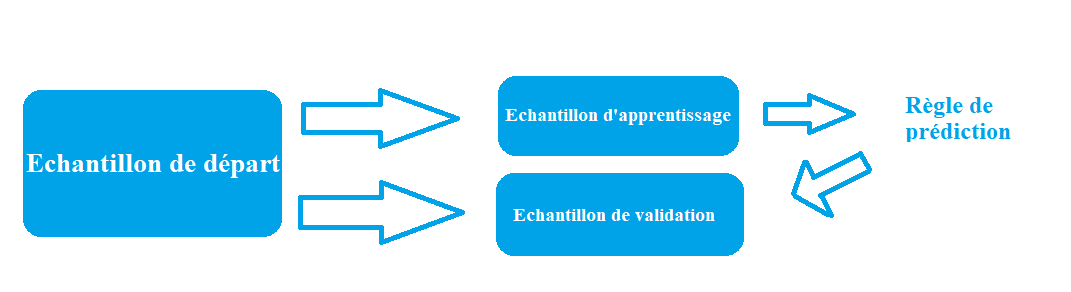
\includegraphics[width=18cm]{Images/hold_out.png}
\begin{center}
\captionof{figure}{Fonctionnement de la validation croisée Hold-Out}
\label{fig1}
\end{center}
\paragraph{}
De façon mathématique, cet estimateur du risque se définit de la façon suivante :
\begin{center}
$\widehat{\mathcal{R}}(f_{D^{n}_{1}}) = \frac{1}{|\mathcal{V}|} \sum\limits_{(x_i,y_i) \in \mathcal{V}} l(y_i,f_{\mathcal{A}}(x_i))$
\end{center}
 avec $|\mathcal{V}|$ le cardinal de $\mathcal{V}$ (autrement dit, le nombre de lignes de l'échantillon de validation) et $f_{\mathcal{A}}(x_i)$ les prédictions de l'algorithme $f$ sur les observations $x_i \in \mathcal{A}$, l'échantillon d'apprentissage.
\paragraph{}
Dans le cadre de nos travaux, l'utilisation de cette méthode va nous permettre de gagner du temps si l'on utilise la matrice de travail contenant toutes les stations. La méthode suivante que nous allons présenter prendra plus de temps mais peut apporter plus de stabilité dans les résultats.
\newpage
\subsubsection{La validation croisée K-Fold}
\paragraph{}
La validation croisée \textbf{K-Fold} est une variante de la méthode vue précédemment, qui on le rappelle était adaptée aux jeux de données de taille suffisamment grande. Cependant sur des jeux de données plus petits, comme c'est le cas de nos fichiers par station qui font environ $27000$ lignes chacun,ce type de validation croisée peut également s'avérer efficace. Le fonctionnement de cette méthode itérative est le suivant :
\begin{itemize}
\item On procède à une partition de notre échantillon en $K$ blocs équilibrés : $B_1,...,B_K$ auxquels sont associés des tailles $n_1,...,n_K$. (En pratique on prend $K=10$ quand la taille des données le permet, sinon on se contente de 5 blocs)
\item On note $d_{B_i}=\{(x_j,y_j), j \in B_i\}$ le $i^{eme}$ bloc  de l'échantillon $d^{n}_{1}$. Pour chaque itération $i = 1,...,K$ on laisse de côté les données de $d_{B_i}$ pour faire notre apprentissage sur les $K$-1 blocs restants
\item On teste la performance de notre règle de prédiction sur le bloc $B_i$ pour obtenir une estimation du risque à l'itération $i$ que l'on note :
\begin{center}
$\widehat{\mathcal{R}}_i = \frac{1}{n_i} \sum\limits_{j \in B_i} l(y_j,f_{d^{n}_{1}\backslash d_{B_i}}(x_j))$
\end{center}
avec $f_{d^{n}_{1}\backslash d_{B_i}}(x_j)$ l'algorithme de prédiction $f$ appliqué aux observations $x_j$ telles que $x_j$ n'appartiennent pas à $d_{B_i}$
\item Enfin, après avoir procédé à toutes les itérations, on calcule la véritable estimation du risque en faisant la moyenne des estimations du risque calculées à chaque itération :
\begin{center}
$\widehat{\mathcal{R}}(f_{D^{n}_{1}}) = \frac{1}{K} \sum\limits_{i=1}^K \widehat{\mathcal{R}}_i$
\end{center}
\end{itemize}
\paragraph{}
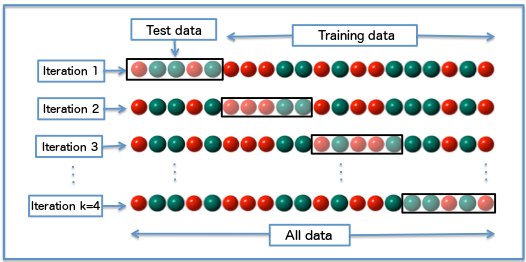
\includegraphics[width=17cm]{Images/k_fold.jpg}
\begin{center}
\captionof{figure}{Exemple de fonctionnement pour K=4}
\label{fig1}
\end{center}
\paragraph{}
Il s'agit désormais d'utiliser la méthode de notre choix dans le but de trouver le meilleur compromis entre précision de l'algorithme et temps de calcul. Le domaine de la \textit{Data Science} fait interagir la théorie mathématique avec la réalisation informatique, il est donc important de prendre en compte ces deux aspects et d'optimiser leur utilisation conjointe au mieux.
\section{Analyse des corrélations entre variables et visualisation}

\subsection{Analyse en Composante Principale}

\paragraph{}
Dans un premier temps nous nous sommes intéressé aux liens existant entre nos variable quantitatives ainsi qu'à leurs importances. Pour cela nous avons réalisé une \textbf{ACP} (Analyse en Composante Principale). Cette technique repose sur la construction d'une représentation à une dimension réduite de nos variables. Le but est donc d'avoir un résumé le plus précis possible, sans modifier les distances entres individus et variables. Pour cela nous projetons notre problème sur des axes représentant une certaine partie de l'inertie de nos données.


\newpage
\section{Travail des données}
\paragraph{}
Avant de lancer différents algorithmes sur nos données, il est important de travailler sur des données \og propres \fg{}. Nous allons donc dans la suite détailler les différentes étapes de nettoyage et de tranformation de certaines données.
\subsection{Gestion et remplacement des valeurs manquantes}
\paragraph{}
Une partie clé de cette étude aura été la gestion des valeurs manquantes. En effet, tous les fichiers $train\_H.csv$ $(H=1,..,36)$, en contiennent, ce qui nous a donc amené à nous poser les questions suivantes : faut-il éliminer les lignes contenant des \textit{NA} ? Faut-il remplacer ces valeurs manquantes ? Si oui, pour quelles variables, de quelle façon et à quel coût ? Nous allons détailler l'analyse qui nous a permis de répondre à ces différentes interrogations et de prendre nos décisions.
\paragraph{}
Premièrement nous avons regardé s'il était possible de remplacer les valeurs sur toutes les variables qui en contiennent dans nos données. Toutes les variables numériques (\textit{i.e} qui ne sont pas des facteurs) présentent des valeurs manquantes. Le graphe suivant nous montre l'erreur moyenne pour chaque variable après des tentatives d'imputation par \textbf{moyenne}, \textbf{médiane}, \textbf{10-NN}, \textbf{Random Forest} et \textbf{décalage temporel} (par exemple s'il manque une valeur pour la variable \textit{ux1H10} à Bordeaux le 20/06/2015 à l'échéance 1, on va remplacer cette valeur par celle de la même date et de la même station à l'échéance 2).

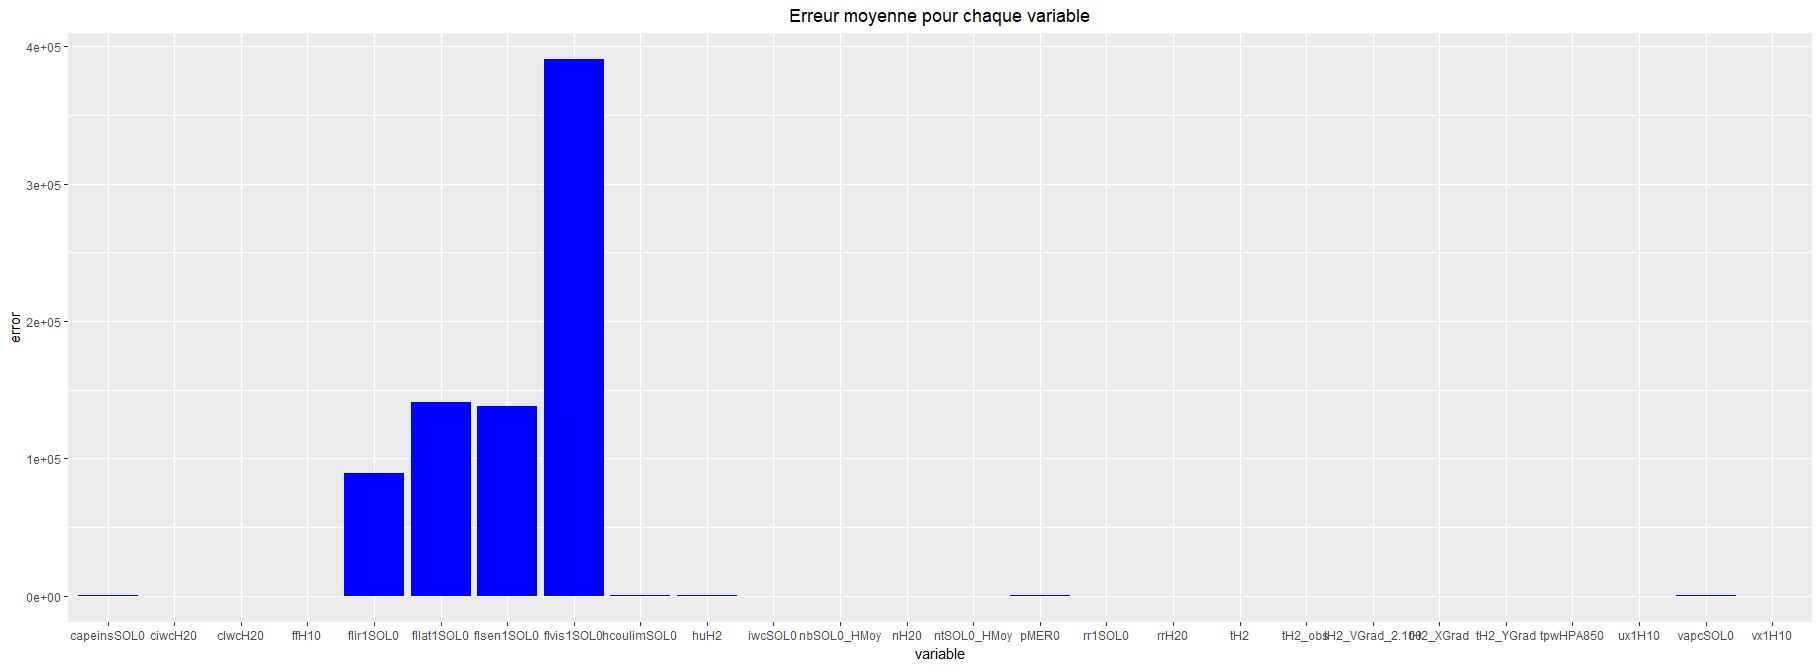
\includegraphics[width=17cm]{Images/na_error.png}
\begin{center}
\captionof{figure}{L'imputation de certaines variables semble problématique}
\label{fig1}
\end{center}
\paragraph{}
Clairement, ce graphique fait ressortir un problème pour les variables \textbf{flir1SOL0}, \textbf{fllat1SOL0}, \textbf{flsen1SOL0}, \textbf{flvis1SOL0} et dans une moindre mesure pour les variables \textbf{hcoulimSOL0} et \textbf{capeinsSOL0}. Nous avons donc décider de ne pas remplacer les valeurs manquantes pour ces variables, puisque les remplacer pourrait potentiellement fausser la qualité de notre analyse.
\paragraph{}
Suite à ce constat, nous allons donc nous pencher plus en détail sur les variables restantes en testant plusieurs méthodes d'imputation de valeurs. Pour réaliser nos tests, nous avons sélectionné les lignes complètes du fichier regroupant les observations pour la station de Toulouse, puis nous avons tiré 2000 lignes de façon aléatoire et sans remise pour former notre échantillon de test. Ensuite, nous avons créé une copie de ce sous-échantillon dans lequel nous avons remplacé 50\% des valeurs par des valeurs manquantes, encore une fois de façon aléatoire. Il ne reste plus qu'à tester différentes méthodes et les comparer.
\newpage
Parmi les méthodes d'imputation essayées, nous retrouvons :
\begin{itemize}
\item L'imputation \textbf{LOCF} (Last Observation Carry Forward) qui est similaire à notre décalage temporel sauf que l'on considère la dernière observation pour effectuer le remplacement
\item L'imputation par la \textbf{moyenne}
\item L'imputation par la \textbf{médiane}
\item L'imputation par les \textbf{k-plus-proches-voisins} ($k=5$ ici)
\item L'imputation \textbf{LOESS} (\textbf{LO}cal regr\textbf{ESS}ion) dont le principe se base sur l'ajustement d'un polynôme de degré faible autour de la donnée manquante par moindres carrés pondérés, en donnant plus de poids aux valeurs proches de la donnée manquante
\item L'imputation par l'algorithme \textbf{SVD} (décomposition en valeurs singulières)
\item L'imputation \textbf{missForest} basée sur les forêts aléatoires, dont le fonctionnement sera détaillé plus loin dans ce rapport
\item L'imputation par l'algorithme \textbf{AMELIA II} : Pour chaque tirage, les données sont estimées par bootstrap pour simuler l'incertitude puis l'algorithme EM est exécuté pour trouver l'estimateur a posteriori $\Theta_{MAP}$ pour les données bootstrap.
\end{itemize}

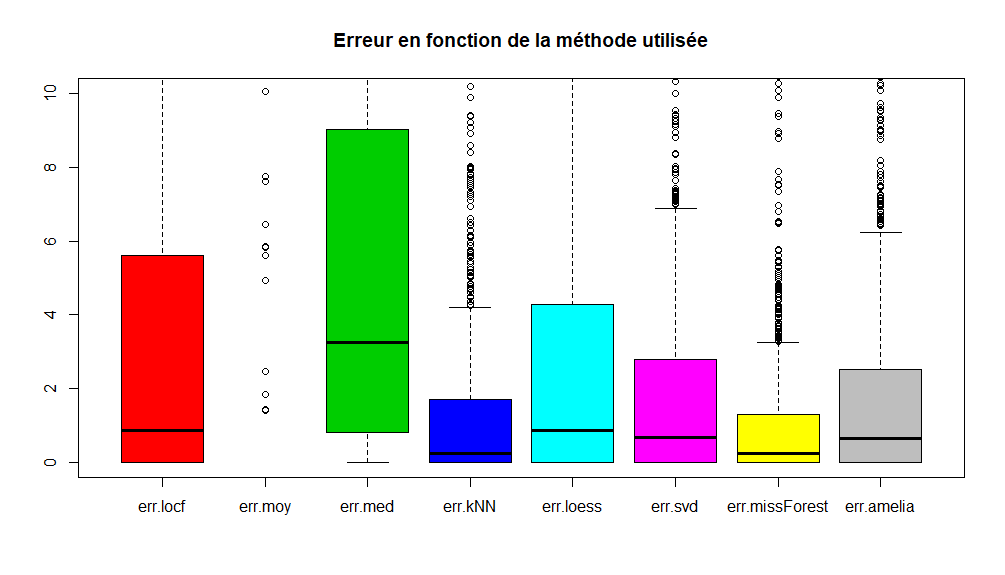
\includegraphics[width=17cm]{Images/err_imp.png}
\begin{center}
\captionof{figure}{Taux d'erreur des méthodes d'imputation testées}
\label{fig1}
\end{center}
\paragraph{}
Le graphe précédent nous permet d'observer que c'est la méthode \textbf{missForest} qui nous procure le moins d'erreur, c'est donc celle-là que nous avons choisi. L'imputation s'est faite par station, pour les raisons exposées dans la partie \og \textbf{Structuration des données} \fg{}.
\newpage 
\subsection{Transformation de la date}
\paragraph{}
Si l'on demandait à une personne de prédire la température, intuitivement la date va forcément faire partie des variables déterminantes dans sa décision. Il paraît évident que l'on ne va pas prédire la même température pour un 15 janvier que pour un 15 juillet. En revanche, on pourrait être tenté de prédire environ la même température pour un 15 avril et pour un 15 octobre, le printemps et l'automne étant assez similaires selon ce critère de température. En revanche, l'été et l'hiver s'opposent. On saisit donc que la variable date va avoir son importance dans l'explication de la température, seulement cette information n'est pas exploitable de façon brute : il va falloir la transformer. Comment choisir cette transformation ? Les critères suivants peuvent nous aider :
\begin{itemize}
\item La transformation doit être capable de représenter l'opposition entre l'hiver et l'été, tout en tenant compte du caractère similaire de l'automne et du printemps
\item Elle doit également prendre en compte le fait que le $31$ décembre d'une année et le $1^{er}$ janvier de l'année suivante sont 2 jours similaires
\item La saisonnalité est un phénomène périodique, il faut donc représenter cet aspect dans la transformation
\end{itemize}
\paragraph{}
Après avoir énuméré ces différents critères, on peut avoir l'intuition que cette transformation à une forme sinusoïdale, plus particulièrement on peut choisir le \textbf{cosinus}. En effet, avec une telle représentation on pourrait respecter tous les critères énoncés précédemment. L'objectif va être d'associer à chaque date une coordonnée qui représente au mieux sa position dans l'année, par exemple quand on se situe au cœur de l'été on aura une coordonnée proche de 1, et inversement au cœur de l'hiver avec -1. Pour effectuer un tel codage, on procède de la façon suivante :
\begin{itemize}
\item on fixe le point de départ au 07/08/2013 : point central de l'été 2013. On attribue 0 comme coordonnée à ce point puisque $cos(0)=1$
\item la coordonnée de la date suivante est incrémentée d'un pas régulier tel que :
\begin{center}
$t_{i+1}=t_{i}+ \frac{2\pi}{N}$
\end{center}
où $N$ correspond au nombre de jours que contient chaque année (cette étude contient une année bissextile dont il a fallu prendre compte)
\item enfin, il ne reste plus qu'à prendre le cosinus de chaque coordonnée et l'on obtient la représentation qui suit :
\end{itemize}
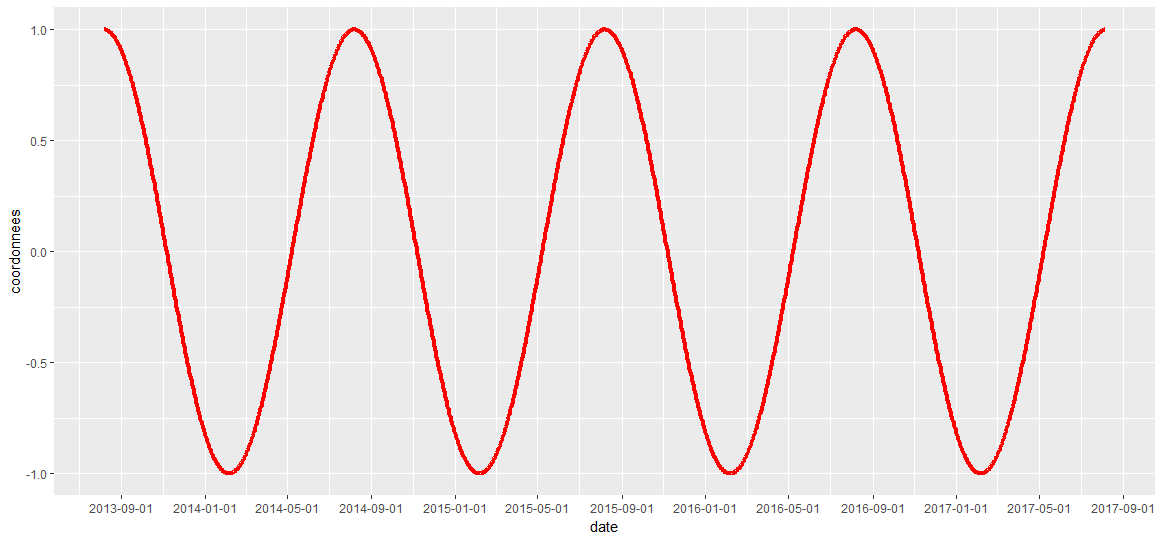
\includegraphics[width=17cm]{Images/date.png}
\begin{center}
\captionof{figure}{A chaque date correspond une coordonnée indiquant sa position dans la saison}
\label{fig1}
\end{center}
\paragraph{}
Les transformations et ajustements étant faits, nous pouvons à présent démarrer la partie de modélisation dans le but de prédire les températures.
\section{Choix et application d'algorithmes d'apprentissage supervisé}
\paragraph{}
Dans cette section, nous allons détailler les différents algorithmes que nous avons utilisé pour modéliser les données et effectuer nos prédictions. Etant donné qu'il n'existe pas une méthode universelle assurant qu'un algorithme est meilleur que les autres pour un type de problème donné, il faut en tester plusieurs (\og No free lunch theorems \fg{}). Toutefois, nous pouvons d'ores et déjà enlever les \textbf{SVM} de la liste des algorithmes qui seront testés. Nous avons fait ce choix pour des raisons techniques : l'algorithme utilise la matrice de Gram définie de la façon suivante :
\begin{center}
$G = \begin{pmatrix} <x_1,x_1> & \cdots & <x_1,x_n> \\ \vdots & \ddots & \vdots \\ <x_n,x_1> & \cdots & <x_n,x_n> \end{pmatrix}$
\end{center}
Cette matrice est de taille $n$ x $n$, ce qui dans le cas de nos données peut poser problème en temps de calcul. Sachant que d'autres méthodes fonctionnant en général très bien et de façon plus rapide sont à notre disposition, nous avons donc décidé de ne pas utiliser l'algorithme \textbf{SVM}. Pour les méthodes testées, le schéma sera le suivant :
\begin{itemize}
\item Présentation du fonctionnement de l'algorithme et de ses propriétés théoriques
\item Présentation des meilleurs résultats obtenus avec l'algorithme et des hyper-paramètres correspondants
\end{itemize}
\paragraph{}
Nous rappelons également au passage que pour optimiser la performance, le critère à minimiser sera l'erreur quadratique moyenne de notre estimateur que l'on peut exprimer de la façon suivante, si l'on note $\hat{\Theta}$ notre estimateur du paramètre $\Theta$ (la température \textbf{tH2\_obs}) :
\begin{center}
$MSE(\hat{\Theta})=\mathbb{E}[(\hat{\Theta}-\Theta)^2]$
\end{center}
Que l'on peut encore décomposer comme étant :
\begin{center}
$MSE(\hat{\Theta})=Biais(\hat{\Theta})^2+Var(\hat{\Theta})$
\end{center}
C'est donc sur ces deux aspects que nous allons tenter de jouer par la suite. Afin d'obtenir la \og meilleure \fg{} performance possible, il faudra trouver le \og meilleur \fg{} compromis biais/variance.
\subsection{Premiers algorithmes : la régression linéaire et ses variantes}

\subsection{Forêt aléatoire : l'algorithme Random Forest}
\subsubsection{Rappels sur le fonctionnement de la méthode CART}
\paragraph{}
Une façon simple de modéliser des données peut être d'utiliser un arbre de décision \textbf{CART} (\textbf{C}lassification \textbf{A}nd \textbf{R}egression \textbf{T}ree). C'est un algorithme de prédiction par moyenne locale, par partition, dont la partition est construite par divisions successives au moyen d'hyperplans orthogonaux aux axes du nœud racine $\mathfrak{X}=\mathbb{R}^{p}$, dépendant des $(X_i,Y_i)$. Chaque division est effectuée à partir du choix conjoint d'une variable explicative et d'une valeur seuil pour cette variable, de sorte que la découpe effectuée minimise la variance en régression ou l'impureté dans le nœud en discrimination.
\begin{center}
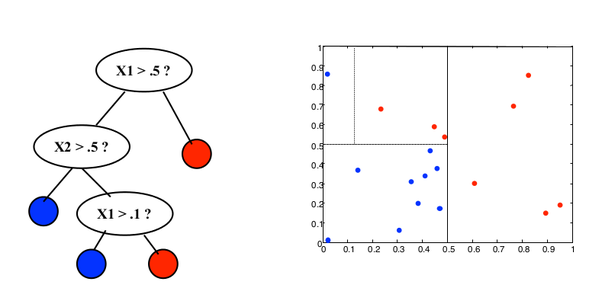
\includegraphics[scale=0.55]{Images/cart.png}
\end{center}
\begin{center}
\captionof{figure}{Illustration de l'algorithme CART pour un problème de discrimination binaire dans $\mathbb{R}^2$}
\label{fig1}
\end{center}
\paragraph{}
Néanmoins cet algorithme pose le problème majeur d'être très instable (fléau de la dimension et sensibilité à l'échantillon). C'est donc pour palier à ce problème que nous allons utiliser l'algorithme de forêt aléatoire \textbf{Random Input}. Comme son nom l'indique, cette méthode consiste en une agrégation d'arbres : c'est un algorithme de \textbf{Bagging} (\textbf{B}ootstrap \textbf{agg}regat\textbf{ing}). 
\subsubsection{Le bagging}
\paragraph{}
Le \textbf{bagging} s'applique à des algorithmes instables, de variance forte, ce qui est le cas des arbres \textbf{CART}. En utilisant un algorithme de \textbf{bagging}, le but va justement être de réduire la variance (quitte à introduire un peu de biais).
En régression, on va agréger \textbf{B} algorithmes $\hat{\eta_1},...,\hat{\eta_B}$ sous la forme :
\begin{center}
$\hat{\eta}(x)=\frac{1}{B}\sum\limits_{b=1}^B \hat{\eta_b}(x)$
\end{center}
Cependant en pratique ces algorithmes ne peuvent pas être i.i.d puisqu'ils sont construits sur le même échantillon $D^{n}_{1}$, et si l'on note $\rho(x)$ le coefficient de corrélation entre $\hat{\eta_b}$ et $\hat{\eta_{b'}}$ on a la relation suivante :
\begin{center}
$Var(\hat{\eta}(x))=\rho(x)Var(\hat{\eta_b}(x))+\frac{1-\rho(x)}{B}Var(\hat{\eta_b}(x))$\\
\medskip
d'où il vient : $\lim_{B \to \infty} Var(\hat{\eta}(x)) = \rho(x)Var(\hat{\eta_b}(x))$
\end{center}
Cela illustre donc le fait que le bagging va réduire la variance de l'estimateur. En revanche, on introduit un terme de corrélation : la solution de \textbf{Breiman} pour construire des algorithmes peu corrélés entre eux consiste à utiliser non pas l'échantillon $D^{n}_{1}$ mais plutôt des échantillons \textbf{bootstrap} de $D^{n}_{1}$, c'est-à-dire que l'on va tirer de façon aléatoire et avec remise des lignes parmi l'échantillon $D^{n}_{1}$.
\subsubsection{L'algorithme Random Forest RI}
L'algorithme de forêt aléatoire Random Input est donc une variante de la méthode CART qui s'appuie sur les techniques de bagging. Son fonctionnement est le suivant :\\
\begin{algorithm}
\caption{Random Forest RI}
\begin{algorithmic}
\REQUIRE 
\STATE $x$ : l'entrée dont on veut prédire la sortie
\STATE $d^{n}_{1}$ : l'échantillon observé
\STATE $m$ : le nombre de variables explicatives sélectionnées à chaque nœud
\STATE $B$ : le nombre d'itérations
\ENSURE
\FOR {b variant de 1 à B}
\STATE Tirer un échantillon bootstrap $d^{*b}$ de $d^{n}_{1}$
\STATE Construire un arbre maximal $\hat{\eta_b}$ sur l'échantillon bootstrap $d^{*b}$ par la variante de CART
\FOR {chaque nœud variant de 1 à $N_b$}
\STATE Tirer un sous-échantillon de $m$ variables explicatives
\STATE Partitionner le nœud à partir de la \og meilleure \fg{} de ces $m$ variables
\ENDFOR
\ENDFOR
\RETURN $\frac{1}{B}\sum\limits_{b=1}^B \hat{\eta_b}(x)$
\PRINT
\end{algorithmic}
\end{algorithm}
\paragraph{}
Il faudra donc calibrer plusieurs hyper-paramètres pour cette méthode : le nombre d'itérations \textbf{B} qui comme on l'a vu précédemment permet de réduire la variance lorsqu'il est grand, et le nombre $m$ de variables explicatives sélectionnées à chaque nœud. Pour cela, nous pouvons utiliser plusieurs méthodes de validation croisée présentées auparavant ou bien encore la méthode \textbf{Out Of Bag} qui consiste à tester l'algorithme sur les observations n'appartenant pas à l'échantillon bootstrap $d^{*b}$ ayant servi à construire l'algorithme de prédiction. En régression, l'erreur Out Of Bag d'une forêt aléatoire RI est définie par :
\begin{center}
$Error_{OOB}=\frac{1}{n}\sum\limits_{i=1}^n (\frac{y_i-\sum\limits_{b=1}^B I_{i}^{b}\hat{\eta_b}(x)}{\sum\limits_{b=1}^B I_{i}^{b}})^2$ où $I_{i}^{b}=1$ si l'observation $i \notin d^{*b}$, 0 sinon
\end{center}
\subsubsection{Résultats obtenus}
\paragraph{}
Les meilleurs résultats pour cette étude ont été obtenus par validation croisée 5-blocs. Le meilleur estimateur pour Toulouse, Nice, Strasbourg et Paris est le suivant :
\begin{verbatim}
RandomForestRegressor(bootstrap=True, criterion='mse', max_depth=None,
           max_features=11, max_leaf_nodes=None, min_impurity_split=1e-07,
           min\_samples_leaf=1, min\_samples_split=2,
           min_weight_fraction_leaf=0.0, n_estimators=800, n_jobs=1,
           oob_score=False, random_state=None, verbose=0, warm_start=False)
\end{verbatim}
Pour les autres stations (Bordeaux, Rennes et Lille) le seul hyper-paramètre qui change est le nombre de variables explicatives sélectionnées à chaque nœud que l'on a appelé $m$ (\textit{max\_features} dans la fonction \textbf{RandomForestRegressor} de la librairie \textit{scikit-learn} en Python) qui vaut 13. Le nombre d'itérations optimal $B$ (ou \textit{n\_estimators} ici) est de 800. Les résultats procurés par cet estimateur sont les suivants :\\
\begin{center}
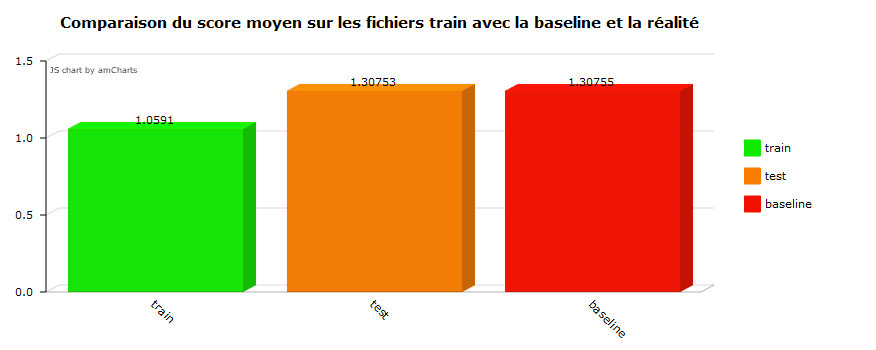
\includegraphics[width=18cm]{Images/score_rf.png}
\end{center}
\begin{center}
\captionof{figure}{Le score de cet algorithme est légèrement meilleur que la baseline}
\label{fig1}
\end{center}
Cet algorithme permet donc de franchir la \textbf{baseline}, cependant on s'aperçoit encore d'un écart important entre le score moyen d'entraînement sur les 7 stations et le score sur le fichier de test. Nous allons maintenant essayer d'autres algorithmes dont le fonctionnement est différent et regarder s'ils nous permettent de gagner en performance.
\subsection{Boosting : l'algorithme XGBoost}
\subsubsection{Rappels sur le fonctionnement du boosting}
\paragraph{}
Le \textbf{boosting}, par opposition au bagging, s'applique à des algorithmes fortements biaisés, mais de faible variance. Le principe est donc bien différent de celui d'une forêt aléatoire où l'on va agréger les prédictions de plusieurs arbres pour en faire la moyenne.
\paragraph{}
Ici on va combiner dans un algorithme itératif les prédictions de \textit{weak learners}, c'est-à-dire des classifieurs ou des régresseurs faibles, selon la nature du problème. Ces prédicteurs faibles sont encore une fois des arbres avec peu de nœuds (pour rester faibles et éviter le sur-apprentissage). 
\paragraph{}
Si l'on se place dans un problème de discrimination, à chaque itérations on va attribuer un poids au classifieur en fonction de sa qualité d'estimation (selon le critère du taux de bon classement par exemple). Les observations qui ont été mal classées se verront attribuer un poids plus fort afin d'être mieux prédites lors de la prochaine itération. La figure suivante résume le fonctionnement de ce type d'algorithmes : chaque \textit{Box} correspond à une itération, et les prédicteurs utilisés sont des arbres à 2 nœuds (encore appelés \textit{stumps}).

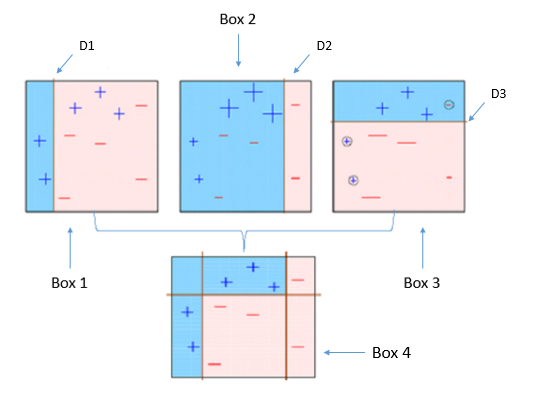
\includegraphics[width=19cm]{Images/boosting.png}
\begin{center}
\captionof{figure}{Illustration du boosting pour un problème de discrimination binaire dans $\mathbb{R}^2$}
\end{center}
\paragraph{}
Il existe énormément de déclinaisons du boosting, dans cet étude nous allons nous focaliser sur un algorithme d'\textbf{eXtreme Gradient Boosting} (XGBoost) régularisé qui s'appuie sur un algorithme de minimisation du risque empirique (fonction de perte \textit{l}) par descente de gradient. Nous avons choisi cet algorithme par rapport à sa popularité que ce soit au niveau des compétitions de type \textit{Kaggle} ou en entreprise (plusieurs soutenances de stage d'élèves de Master 2 parlaient de cette méthode en 2016), mais également pour sa rapidité à être implémenté. La version régularisée doit nous permettre d'éviter, ou en tout cas de limiter le sur-apprentissage.
\subsubsection{Descente de gradient stochastique}
\paragraph{}
Avant d'expliquer le fonctionnement de l'algorithme \textbf{XGBoost} il est primordial d'effectuer un rappel sur l'algorithme d'optimisation qui en est la base : la descente de gradient. Nous avons même fait le choix d'utiliser une descente de gradient stochastique (on ne regarde qu'une partie des observations pour effectuer la mise à jour du gradient). Cela a pour propriété de réduire la variance moyennant une augmentation du biais, mais les éléments de littérature laissent à penser que la réduction de variance est plus importante que l'introduction de biais, et que cela permet donc d'améliorer la performance de l'algorithme de prédiction. Dans le cas simple où l'on cherche à minimiser une fonction convexe, on se fixe un point de départ et on \og descend \fg{} le long de cette fonction en la différenciant jusqu'à atteindre le minimum global.
\begin{center}
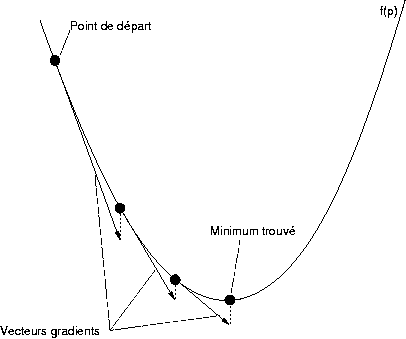
\includegraphics[scale=0.7]{Images/descente.png}
\end{center}
\begin{center}
\captionof{figure}{Descente de gradient sur une fonction convexe simple dans le plan}
\end{center}
\paragraph{}
Cependant, un paramètre essentiel à choisir dans cette méthode va être le \textbf{pas de descente}. Un pas trop grand va mener à une irrégularité et à des résultats très mauvais car le minimum ne sera jamais atteint.\\
Au contraire, un pas trop petit va premièrement avoir pour effet de ralentir le temps de calcul de l'algorithme, et deuxièmement nous exposer au risque de ne jamais atteindre le minimum si l'on s'arrête trop tôt au niveau du nombre d'itérations de l'algorithme.
\begin{center}
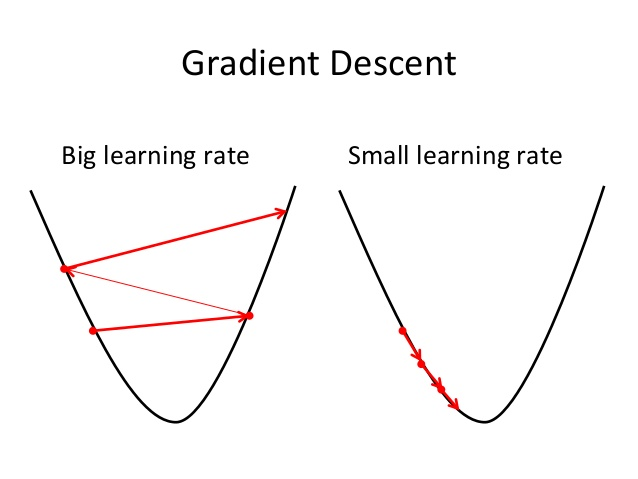
\includegraphics[scale=0.5]{Images/lr.jpg}
\end{center}
\begin{center}
\captionof{figure}{Problème : le choix du pas est crucial}
\end{center}
\paragraph{}
Cela nous permet déjà de nous rendre compte que le nombre d'itérations de l'algorithme et le pas (learning rate) sont deux paramètres qui vont être liés et qui seront cruciaux dans la quête du minimum global de la fonction de perte qu'on cherche à atteindre, et donc pour la qualité d'estimation. En revanche, les cas présentés ci-dessus sont des cas simples, où la fonction est convexe. Une difficulté supplémentaire en pratique va souvent être que la fonction de perte que l'on cherche à minimiser ne sera pas convexe.
\begin{center}
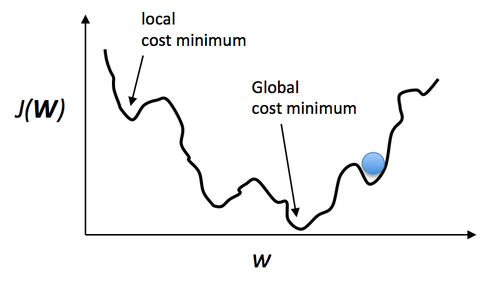
\includegraphics[scale=0.7]{Images/nonconvex-cost.png}
\end{center}
\begin{center}
\captionof{figure}{Dans la pratique on se retrouve plus souvent confronté à ce type de fonctions}
\end{center}
\paragraph{}
L'enjeu va donc être de choisir un nombre d'itérations et un pas optimal afin de ne pas se retrouver \og coincé \fg{} dans un minimum local et de pouvoir atteindre le minimum global de la fonction de perte qu'on souhaite minimiser. Une autre solution plus complexe pourrait être de chercher un majorant convexe de la fonction de perte et de chercher à le minimiser. Ce principe est par exemple utilisé dans le cadre d'une SVM où l'on procède à une minimisation du risque empirique convexifié régularisé. 
\subsubsection{Fonctionnement du Gradient Boosting régularisé}
\paragraph{}
Dans cette partie, nous allons exprimer le fonctionnement de cette méthode de façon algorithmique puis en détailler les étapes afin de bien comprendre le traitement effectué par cette opération. L'algorithme de gradient boosting régularisé en régression peut s'écrire de la façon suivante :\\
\begin{algorithm}
\caption{Gradient Boosting régularisé}
\begin{algorithmic}
\REQUIRE 
\STATE $\phi_{\gamma}$ : algorithme faible de paramètre $\gamma$ à ajuster
\STATE $\lambda \in $ $]0,1]$ : paramètre de régularisation\\
\ENSURE
\STATE Initialiser $\hat{\eta}^0(x)=\underset{c}{argmin}\sum\limits_{i=1}^n l(y_i,c)$
\FOR {b variant de 1 à B}
\STATE Calculer $z_{i}^b=-\frac{\partial}{\partial_{\eta(x_i)}}l(y_i,\eta(x_i))\vert_{\eta(x_i)=\hat{\eta}^{b-1}(x_i)}$
\STATE Ajuster $\hat{\gamma}^b=\underset{\gamma}{argmin}\sum\limits_{i=1}^n(z_{i}^b-\phi_{\gamma}(x_i))^2$
\STATE Calculer $\hat{\beta}_b=\underset{\beta}{argmin}\sum\limits_{i=1}^n l(y_i,\hat{\eta}^{b-1}(x_i)+\beta\phi_{\hat{\gamma}^b}(x_i))$
\STATE Mettre à jour $\hat{\eta}^b(x)=\hat{\eta}^{b-1}(x)+\lambda\beta\phi_{\hat{\gamma}^b}(x)$
\ENDFOR
\RETURN $\hat{\eta}^B$
\PRINT
\end{algorithmic}
\end{algorithm}
\paragraph{}
Nous allons à présent reprendre ces écritures afin de mieux comprendre les tâches effectuées par l'algorithme. Premièrement décrivons les entrées de cet algorithme :
\begin{itemize}
\item $\phi_{\gamma}$ va correspondre dans notre étude à un arbre. $\gamma$ sera par exemple le nombre de nœuds de cet arbre que l'on ajustera par validation croisée 5-blocs encore une fois
\item $\lambda$ est l'hyper-paramètre qui va nous permettre d'effectuer de la régularisation. On l'appelle également le \textit{learning rate}, c'est ce que nous avons décrit précédemment comme étant le pas de descente de gradient. Puisque $\lambda \in$ $]0,1]$ on voit donc qu'il réduit/limite l'apprentissage de chaque itération, ce qui doit nous aider à nous prémunir contre le risque de sur-apprentissage
\end{itemize}
On entre ensuite au cœur du problème d'optimisation, qui dans le cas de la méthode \textbf{XGBoost} s'appuie sur une minimisation du risque empirique par descente de gradient. Cela implique également le choix d'une fonction de perte $l$. Comme expliqué précédemment :
\begin{itemize}
\item on choisit un point de départ lors de l'initialisation, puis on procède à la descente de gradient (dans la direction de plus forte descente correspondant à $z_{i}^b$) dans le but de minimiser $l$
\item on met à jour les poids en fonction de la qualité de prédiction du \og prédicteur faible \fg{}
\item on actualise la prédiction $\hat{\eta}^b(x)$ de l'itération en fonction de la prédiction de l'itération précédente et de l'apprentissage effectué au cours de l'itération actuelle
\item A la fin des \textbf{B} itérations que l'on s'est fixé, on renvoie la dernière prédiction.
\end{itemize}
Comme introduit précédemment, le nombre d'itérations \textbf{B} et le learning rate \textbf{$\lambda$} sont deux hyper-paramètres qui interagissent et qu'il va donc falloir calibrer de façon simultanée. Cet ajustement va se faire par validation croisée 5-blocs et on va fixer l'un des paramètres en faisant varier l'autre. En ce qui nous concerne, le nombre d'itérations sera fixé et c'est le learning rate qui va varier.

\subsubsection{Résultats obtenus}
\paragraph{}
La sortie en Python correspondant au meilleur estimateur, que nous allons détailler, est la suivante :
\begin{verbatim}
GradientBoostingRegressor(alpha=0.9, criterion='friedman_mse', init=None,
             learning_rate=0.05, loss='ls', max_depth=8, max_features=None,
             max_leaf_nodes=None, min_impurity_split=1e-07,
             min_samples_leaf=1, min_samples_split=2,
             min_weight_fraction_leaf=0.0, n_estimators=1200,
             presort='auto', random_state=None, subsample=0.9, verbose=0,
             warm_start=False)
\end{verbatim}
\paragraph{}
Les hyper-paramètres optimaux sont les mêmes pour toutes les stations, parmi ceux qui ont été choisis et ajustés (\textit{i.e} pas laissés par défaut), on retrouve :
\begin{itemize}
\item un nombre d'itérations (\textit{n\_estimators}) de $1200$ associé à un pas de descente (\textit{learning\_rate}) de $0.05$
\item la fonction de perte (\textit{loss}) classique, à savoir \og ls \fg{} pour \textit{least squares regression}. La fonction \textbf{Huber} réputée plus robuste dans certains articles n'apportait pas plus de performance
\item une profondeur d'arbre (\textit{max\_depth}) de 8. On souhaite garder un arbre peu profond afin qu'il reste faible et qu'on évite le sur-apprentissage, cependant les \textit{stumps} (arbres à 2 nœuds) procuraient de moins bons résultats finaux.
\item une proportion d'observations (\textit{subsample}) utilisées pour effectuer les mises à jour de gradient de $0.9$ : c'est ce paramètre qui permet d'effectuer une descente de gradient stochastique
\end{itemize}
Les résultats obtenus grâce à cet estimateur sont les suivants :\\
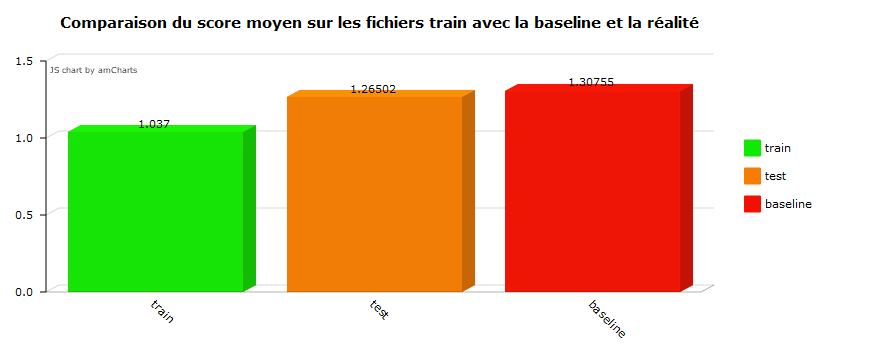
\includegraphics[scale=0.8]{Images/score_boosting.png}
\begin{center}
\captionof{figure}{La performance est meilleure par rapport aux algorithmes précédents}
\label{fig1}
\end{center}
\subsection{Deep Learning : l'utilisation des réseaux de neurones}

\subsubsection{Le contexte}
\paragraph{}
Le Deep Learning permet de résoudre différents problèmes que nous pouvons rencontrer avec les réseaux de neurones comme la stabilité. Aujourd'hui il est souvent utilisé pour des problèmes divers avec des résultats parfois remarquables comme nous pouvons le voir avec le site de traduction \textit{DeepL}, le plus abouti aujourd'hui pour le grand public ou encore pour des outils d'analyse des émotions par un visage photographié ou filmé.

\subsubsection{Le principe}
Le principe de base du modèle (montré dans l'image ci-dessous) est le neurone, un modèle d'inspiration biologique du neurone humain. Chez l'homme, les différents niveaux de puissance des signaux de sortie des neurones circulent le long des jonctions synaptiques et sont ensuite agrégés en entrée pour l'activation d'un neurone connecté. On appelle ce modèle le modèle \textbf{perceptron}.

\begin{center}
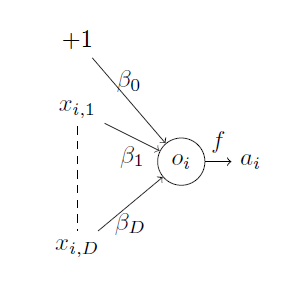
\includegraphics[scale=0.7]{Images/perceptron.png}
\end{center}

Dans le modèle, la fonction f représente la fonction d'activation non linéaire utilisée dans tout le réseau et le biais $\beta_{0} $ représente le seuil d'activation du neurone :
\begin{center}
$y_{i}=f(\beta_{0} + \sum\limits_{j} \beta_{j}x_{i,j}) + \varepsilon_{i}$
\end{center}

\paragraph{}
Une fois que nous avons choisi notre fonction d'activation, il est nécessaire comme dans tout problème d'optimisation de se fixer une fonction de coût à minimiser. Il s'agit ici d'un problème de descente de gradient comme vu précédemment dans la partie sur le Boosting.

\begin{center}
$L(\beta)=\sum\limits_{i}(y_{i}-a_{i})^{2}=\sum\limits_{i}(\beta)$
\end{center}

Il ne reste plus qu'à exprimer le gradient de cette fonction de coût et choisir un pas $\eta$ pour effectuer les mises à jour.

\paragraph{}
Les réseaux neuronaux multicouches en aval sont constitués de plusieurs couches d'unités neuronales interconnectées (comme le montre l'image suivante), commençant par une couche d'entrée pour correspondre à l'espace d'entrée (le nombre de variables), suivie de plusieurs couches non-linéaire, et se terminant par une régression linéaire ou une couche de classification pour correspondre à l'espace de sortie (une régression linéaire dans notre cas). Les entrées et les sorties des unités du modèle suivent la logique de base du neurone décrite ci-dessus.

\begin{center}
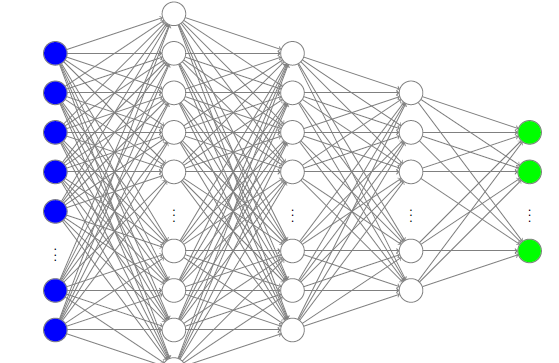
\includegraphics[scale=0.7]{Images/RN.png}
\end{center}

\paragraph{}
Les poids reliant les neurones et les biais avec d'autres neurones déterminent entièrement la sortie de l'ensemble du réseau. L'apprentissage se produit lorsque ces poids sont adaptés pour minimiser l'erreur sur les données d'entraînement marquées.

\subsubsection{Notre premier réseau de neurones}

\paragraph{}
Nous avons réalisé notre premier réseau de neurones rapidement dans la compétition en parallèle des autres méthodes essayées. Pour cela nous avons utilisé le package $H2O$ sous $R$. Nous avons pu tester un premier algorithme de Deep Learning sans grille pour comprendre tous les paramètres et hyper-paramètres qui vont rentrer en jeu ensuite pour avoir un résultat le plus poussé possible. Avec le package $H2O$ nous dénombrons plus de $60$ arguments. Quels arguments choisir et comment?

\begin{verbatim}
model <- h2o.deeplearning(x=predictors, y=response,training_frame=train,
validation_frame=valid,stopping_metric="RMSE",
stopping_tolerance=1e-7,activation="RectifierWithDropout",hidden=c(128,128,64), 
epochs=500,l1=1e-7,stopping_rounds=100,rate=0.0001,
hidden_dropout_ratios=c(0.2,0.2,0.2))
\end{verbatim}

Pour notre premier essai sur un réseau de neurones nous avons choisi un modèle simple à 3 couches cachées. Le modèle est effectué à l'aide d'une validation croisée \textbf{Hold-Out}  $80-20$ pourcent avec un nombre d'epochs à 500.



\begin{itemize}
\item Le nombre d'\textit{epochs} spécifie le nombre d'itérations sur le jeu de données d'entraînement.
\item \textit{Stopping metric} correspond à la métrique employée pour utiliser un \textit{early stopping}. Cela permet d'arrêter notre descente de gradient quand la tolérance relative de l'arrêt métrique pour arrêter la formation (si amélioration) est inférieure à cette valeur, ici c'est notre \textit{stopping tolerance}.
\item \textit{Stopping Rounds}; le nombre d'itérations avant d'arrêter l'algorithme si nous avons convergence.
\item  \textit{Activation} nous permet de choisir la fonction d'activation des neurones du réseau, ici c'est la fonction d'activation \textit{ReLU} (rectified linear unit).
\item \textit{l1}, spécifie la régularisation l1 (L1 = lasso) qui contraint la valeur absolue des poids (peut ajouter de la stabilité et améliorer la généralisation, entraîne de nombreux poids à devenir 0).
\item \textit{Rate} permet de sélectionner le taux d'apprentissage $\alpha$.  Des valeurs plus élevées conduisent à des modèles moins stables, tandis que des valeurs plus faibles entraînent une convergence plus lente.
\item \textit{Hidden dropout ratios} va permettre de diminuer le sur-apprentissage en omettant une fraction de chaque couche cachée.
\end{itemize}

\begin{center}
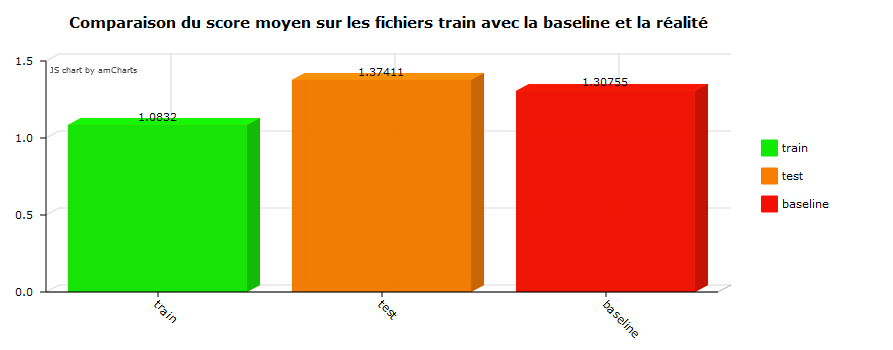
\includegraphics[scale=0.7]{Images/deep1h2o.png}
\end{center}

\paragraph{}
La première difficulté réside dans le fait de choisir notre réseau, un réseau avec beaucoup de couches sera-t-il meilleur pour notre problème ? Un réseau avec des couches larges est généralement meilleur pour l'apprentissage mais à partir de quel moment sommes-nous dans le \textit{sur-apprentissage} ?


\subsubsection{Optimisation du choix des paramètres pour un réseau de neurones sous H2O}

\paragraph{}
Une fois notre premier modèle effectué nous avons eu pour objectif d'avoir un modèle correspondant à notre problème. Pour une raison de temps et d'efficacité nous avons décidé de fixer certains paramètres tandis que d'autres rentreront dans une grille, ils seront nos hyper-paramètres à optimiser.

\begin{verbatim}
    hyper_params <- list(
    hidden=list(c(32,32,32),c(64,64)),
    input_dropout_ratio=c(0,0.05),
    rate=c(0.01,0.02),
    rate_annealing=c(1e-8,1e-7,1e-6))
\end{verbatim}

\paragraph{}
Nous utilisons les paramètres vu dans le premier modèle complété par un \textbf{rate annealing}, son but est de diminuer le taux d'apprentissage (rate) au cours de l'avancement de l'algorithme. Ce paramètre permet de gagner du temps en ayant une plus forte descente de gradient au départ afin de se rapprocher de la zone du minimum, puis ensuite en diminuant le pas au fur et à mesure de l'avancement, d'atteindre le minimum global. Cette technique suit le même principe que la dichotomie.

\paragraph{}
Pour notre modèle nous avons fixé certains paramètres :
\begin{itemize}
    \item \textbf{epochs}, le nombre d'epochs est surtout un choix pour la rapidité du modèle, un grand nombre d'epochs sera toujours favorable.
    \item la régularisation \textbf{l1}.
    \item le paramètre \textbf{max w2}, il spécifie le maximum pour la somme des poids carrés entrants d'un neurone. C'est particulièrement utile quand nous utilisons une fonction d'activation telle que Rectifier (ReLU), cela permet d'éviter d'avoir trop de poids sur un neurone et de mieux répartir l'information.
    \item \textbf{Momentum start}, l'ajout du paramètre de momentum permet de stabiliser l'apprentissage, tout en augmentant la descente de la courbe de la somme des erreurs carrées (fonction de perte) selon les itérations.
\end{itemize}

\paragraph{}
Cette grille nous a permis de déterminer le modèle le plus adapté parmi ceux proposés :

\begin{verbatim}
    model <- h2o.deeplearning(x=predictors, 
                          y=response,
                          training_frame=train,
                          validation_frame=valid,
                          stopping_metric="RMSE",
                          stopping_tolerance=1e-3,
                          activation="RectifierWithDropout",
                          hidden=c(64,64),
                          input_dropout_ratio=0.05,
                          epochs=500, l1=1e-5,stopping_rounds=100,
                          rate=0.01,rate_annealing=1e-7)
\end{verbatim}

\begin{center}
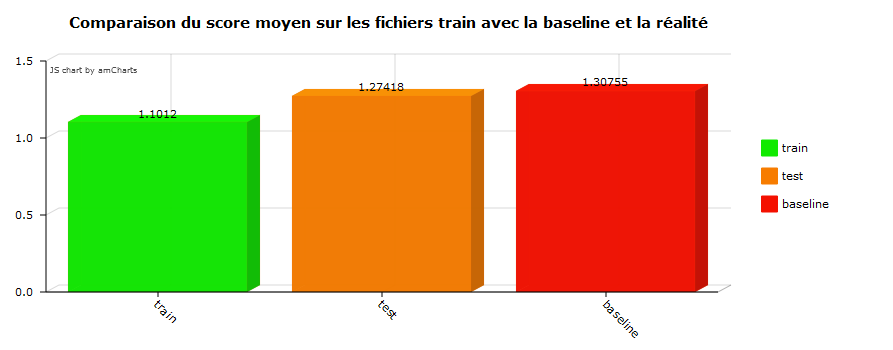
\includegraphics[scale=0.7]{Images/deeph2o.png}
\end{center}


\paragraph{}
Avec ce modèle nous avons atteint notre meilleur score pendant 1 mois mais là est apparu une limite, en essayant d'améliorer notre modèle nous passions à chaque fois dans de l'overfitting.

\subsection{Passage sous Keras}

\paragraph{}
Suite à cette stagnation, nous avons décidé d'appliquer le cours de Mr Tavenard sur les réseaux de neurones en utilisant la bibliothéque \textit{Keras} sous python.

\subsubsection{Premier modèle sous Keras}
\paragraph{}
Pour réaliser notre premier réseau sous \textit{Keras}, nous avons utilisé nos données sans les variables \textit{capeinSOL0} et \textit{rr1SOL0} ainsi que la transformation sinusoïdale sur les dates. Cela nous permet une fois les valeurs manquantes enlevées d'avoir $177977$ individus sur $189280$ ainsi nous limitons la perte de données et cela nous permet de ne pas insérer du biais en faisant une estimation sur les valeurs non présentes.

\paragraph{}
Python et les data.frame \textit{pandas} ne prennent pas en compte les variables catégorielles de la même façon, là ou en \textit{R} il suffit de passer la colonne en facteur, sur \textit{Python} nous devons transformer notre data.frame en tableau disjonctif.

\begin{quote}
    Exemple de la transformation :
\end{quote}
\begin{center}
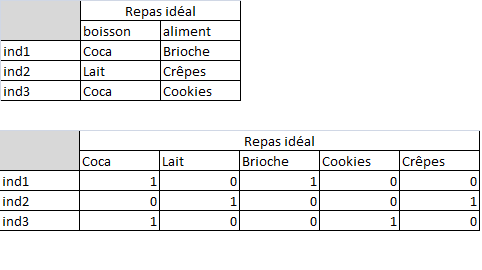
\includegraphics[scale=0.7]{Images/tableaudisjonctif.png}
\end{center}

\paragraph{}
Nous nous retrouvons donc avec un data.frame au dimension suivante $1777977x72$ et notre variable cible $1777977x1$. Puis dans un second temps nous standardisons nos variables explicatives pour le jeu de données train et test, pour cela on standardise d'abord notre jeu d'apprentissage puis nous appliquons la même transformation au jeu de test.

\paragraph{}
Notre premier modèle se veut simple et compréhensible afin d'effectuer nos premiers test sous \textit{Keras}. Pour cela nous prenons un modèle à $1$ couches cachées, nous incluons aussi un DropOut de ces couches pour limiter le sur-apprentissage comme sous \textit{H2O}, la fonction d'activation ReLU ainsi qu'un learning rate de $0.0001$.

\begin{verbatim}
premiere_couche = Dense(units=100, activation="relu", input_dim=72)
couche_cachee1 = Dense(units=100, activation="relu")
couche_sortie = Dense(units=1)
opti = RMSprop(lr=0.0001)

def baseline_model():
    model = Sequential()
    model.add(premiere_couche)
    model.add(Dropout(0.02, noise_shape=None, seed=None))
    model.add(couche_cachee1)
    model.add(Dropout(0.02, noise_shape=None, seed=None))
    model.add(couche_sortie)
    model.compile(optimizer=opti, loss="mean_squared_error")
    return model
    
model = baseline_model()
hist = model.fit(X_train,y_train,
validation_split=0.3,epochs=500,batch_size=500,verbose=2)
\end{verbatim}

\begin{center}
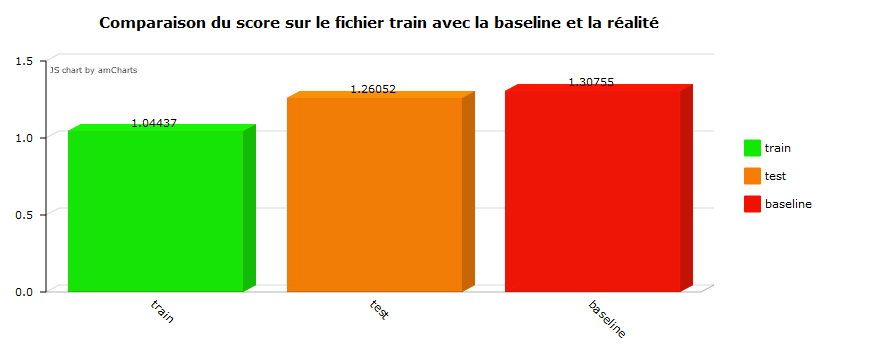
\includegraphics[scale=0.7]{Images/deep1keras.png}
\end{center}

\paragraph{}
Ce modèle nous a permis d'améliorer notre précèdent meilleur score et d'envisager des améliorations.

\subsubsection{Notre meilleur score}
\paragraph{}
Suite à ce modèle nous décidâmes de réutiliser le même modèle avec un data.frame enrichi. Plusieurs pistes ont été envisagées puis testées :
\begin{itemize}
    \item Rajouter les coordonnées de l'ACP précédemment calculées,
    \item Rajouter les coordonnées de l'ACM sur nos jeux de données,
    \item Rajouter des variables par intéractions.
\end{itemize}

\paragraph{}
Le but étant de rajouter de l'information à nos jeux de données en ajoutant des variables même si elles sont corrélées aux variables initiales en prenant le principe simple de la grande dimension :
\begin{quote}
    "Rajouter de l'information ne sera jamais préjudiciable, dans le meilleur des cas nous améliorons notre score, dans le pire nous n'améliorons pas notre modèle mais nous ne le pénalisons pas non plus.
\end{quote}
\paragraph{}
La complexité reposera principalement sur le fait de réussir à adapter notre modèle aux nouvelles variables.

\paragraph{}
\textbf{Premièrement} nous allons ajouter les coordonnées des individus sur les principaux axes de l'ACP. Cette manoeuvre sera composé de plusieurs étapes :
\begin{itemize}
    \item Effectuer une ACP sur le jeu de données train sans la variable cible.
    \item Récupérer les coordonnées des individus sur les axes représentant $80$ pourcent de l'inertie, au delà nous considérons que c'est du bruit.
    \item Projeter nos individus du jeu test sur nos axes calculés précédemment.
\end{itemize}

\paragraph{}
Avec ce procédé nous agrémentons nos jeux de données de 11 variables correspondant aux axes représentant $82$ pourcent de l'inertie. Nous effectuons le même modèle que précédemment en adaptant la dimension d'entrée du réseau, en passant de $72$ à $83$. Les résultats dépassent nos premières attentes :

\begin{center}
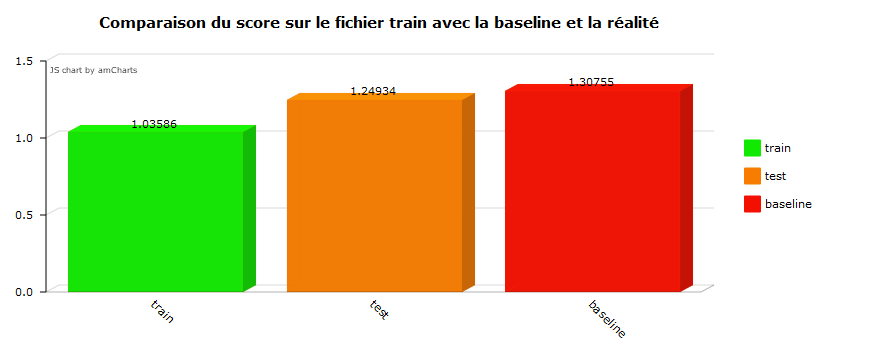
\includegraphics[scale=0.7]{Images/deep2keras.png}
\end{center}

\paragraph{}
\textbf{Deuxièmement} nous allons compléter nos data.frames avec les coordonnées de l'ACM (sur les données qualitatives). Pour la réalisation de cette étape nous procédons de la même façon.

\paragraph{}
Lors de la réalisation de cette ACM, les premiers axes portent peu d'inertie ce qui implique que pour avoir $80$ pourcent de l'inertie nous devons prendre les $44$ premiers axes. Nous rajoutons ces $44$ variables aux données déjà complété par les coordonnées de l'ACP.

\paragraph{}
En adaptant les dimensions d'entrées du réseau de neurones, lors de l'avancement du réseau nous apercevons un décrochage entre le score (RMSE) de la partie apprentissage et la partie validation. Ce décrochage est synonyme de sur-apprentissage, cela se valide sur le jeu de données test comme nous pouvons le voir ci-dessous.

\begin{center}
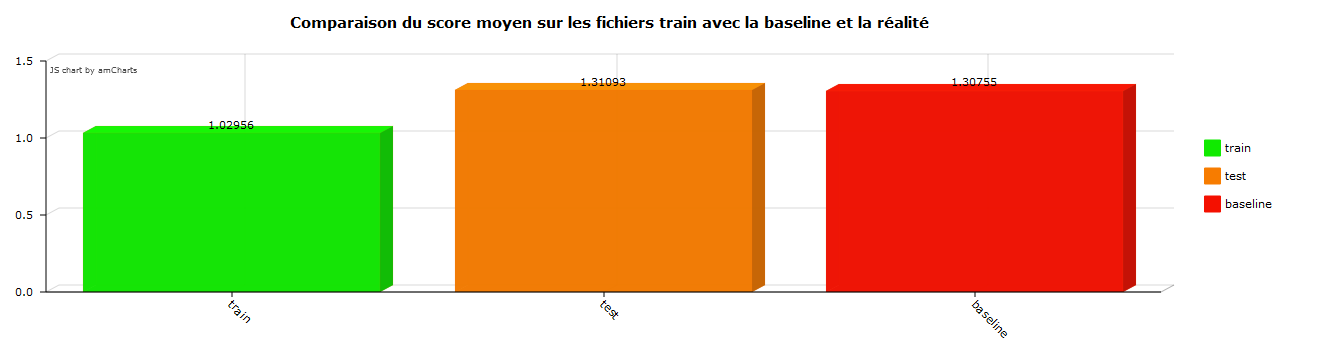
\includegraphics[scale=0.5]{Images/deepacm.png}
\end{center}

\paragraph{}
Le modèle n'est plus adapté et l'information apportée par les axes de l'ACM est trop faible. Par conséquent on ne retient pas cette méthode.

\paragraph{}
\textbf{Troisièmement} nous procédons à la création de nouvelles variables par interaction en réalisant le produit de chaque variable quantitative et explicative avec les autres.

\paragraph{}
La création de nouvelles variable peut permettre d'utiliser le lien qu'il existe entre les variables. Nous agrémentons notre jeu de données de $600$ nouvelles variables.

\paragraph{}
La limite de cette méthode apparaît rapidement lors de nos premiers réseaux, on note un fort décalage entre le score sur la partie \textit{train} et la partie \textit{valid}. Nous sommes clairement dans de \textbf{l'overfitting}.

AJOUTER PHOTO COURBE TRAIN VALID

\paragraph{}
\textbf{En conclusion} nous prenons la décision de ne garder que nos data.frame enrichi des coordonnées des $11$ premiers axes de l'ACP.

\subsubsection{Optimisation de notre meilleur modèle}
\paragraph{}
Le modèle ayant obtenu le meilleur score possède des paramètres choisis arbitrairement. Nous allons donc essayer de faire varier différents paramètre en les incluant dans une grille. Pour effectuer le choix nous utiliserons une validation croisée \textit{5-folds}. Nous incluons aussi un \textit{early-stopping} afin de garder en mémoire le meilleur score lors de la descente de gradient et non la dernière itération comme précédemment.

\paragraph{}
On fait varier la \textit{longueur} et la \textit{largeur} du réseau.
\begin{verbatim}
    dict_params = {'lst_neurals' : [[100,100,64],[300,300,100],[200,200,100,50]]}
\end{verbatim}

\paragraph{}
L'algorithme choisi finalement le réseau initial $100-100-64$ par rapport à un modèle plus large ou plus profond. Pour conclure notre meilleur modèle est donc celui-ci:

\begin{verbatim}
REFAIRE TOURNER UN CODE 
\end{verbatim}

\subsubsection{Conclusion sur le Deep Learning/Réseau de neurones (à mettre dans le BILAN ??)}
\paragraph{}
Le principal point positif des réseaux de neurones dans notre étude est le fait d'avoir réussi à atteindre nos meilleurs scores sur des réseaux simples sans avoir à effectuer beaucoup de transformations sur nos données. La première analyse d'un réseau est simple et visuel cependant l'effet \textbf{boite noire} apparaît rapidement, nous ne pouvons aujourd'hui expliquer par quelles raisonnement ces algorithmes nous permet d'avoir de bons scores. Nous savons ce qu'il se passe à l'entrée du réseau, connaissons la sortie du réseau mais le parcours entre les deux nous est inconnue.

\paragraph{}
Cet effet boite noire ne nous permet pas d'avoir de réel argument pour choisir nos paramètres à optimiser. \textbf{L'overfitting} est toujours très proche de ces méthodes quand nous testons des réseaux plus complexes. Un point négatif supplémentaire est le côté "chronophage" de cette méthode.

\section{Bilan}

\section{Bibliographie et sources}

\begin{flushleft}
- \textbf{WikiStat}, \href{https://www.math.univ-toulouse.fr/~besse/Wikistat/pdf/st-scenar-app-idm.pdf}{\textit{\textcolor{blue}{Scénario: Imputation de données manquantes}}}\\
\medskip
- \textbf{Documentation de scikit-learn}, \href{http://scikit-learn.org/stable/supervised_learning.html#supervised-learning}{\textit{\textcolor{blue}{Librairies pour faire de l'apprentissage supervisé en Python}}}\\
\medskip
- \textbf{Jason Brownlee}, \href{https://machinelearningmastery.com/gentle-introduction-gradient-boosting-algorithm-machine-learning/}{\textit{\textcolor{blue}{A Gentle Introduction to the Gradient Boosting Algorithm for Machine Learning}}}\\
\end{flushleft}

\end{document}
